% =============================================================================
% COPYRIGHT AND DISCLAIMER
% =============================================================================
% This file is provided as a convenience template for competition participants.
% By using it, you accept full responsibility for compliance with all applicable
% copyright, licensing, and usage rules of the Association for Computing
% Machinery (ACM) and of any LaTeX packages you load (including, without
% limitation, the "acmart" document class and related ACM materials).
%
% Consult ACM's official publication, template, and copyright policies before
% using this setup for any purpose other than this competition. Do not assume
% that this template may be reused, redistributed, or submitted elsewhere
% without independently verifying ACM's current rules.
%
% Use of the "acmart" class, the "sigconf" option, or ACM-style formatting in
% this template does NOT mean that this report, this competition, its organizers,
% or any resulting PDF is sponsored, endorsed, affiliated with, or published by
% ACM. ACM trademarks and branding remain the property of ACM.
%
% Template packages live in preamble.tex.
% Citations live in main.bib. Edit this file with your paper content.
% =============================================================================

\documentclass[sigconf]{acmart}
% =============================================================================
% Template setup — participants normally do not edit this file.
% Author content belongs in main.tex; citations belong in main.bib.
% \documentclass lives in main.tex so Overleaf does not treat this file as root.
% =============================================================================

% --- Competition / non-ACM-submission friendly rights metadata -------------
\setcopyright{none}
\settopmatter{printacmref=false}
\acmConference[Kaggle Competition]{Filament Segmentation Challenge}{2026}{\href{https://www.kaggle.com/competitions/filament-segmentation-2026}{kaggle.com/competitions/filament-segmentation-2026}}
\acmBooktitle{Competition Report}
\acmDOI{}
\acmISBN{}

% --- Author guidance text --------------------------------------------------
% \guide{...} is gray italic while \guideStyletrue; omitted from the PDF if false.
% Flip the switch in main.tex after % =============================================================================
% Template setup — participants normally do not edit this file.
% Author content belongs in main.tex; citations belong in main.bib.
% \documentclass lives in main.tex so Overleaf does not treat this file as root.
% =============================================================================

% --- Competition / non-ACM-submission friendly rights metadata -------------
\setcopyright{none}
\settopmatter{printacmref=false}
\acmConference[Kaggle Competition]{Filament Segmentation Challenge}{2026}{\href{https://www.kaggle.com/competitions/filament-segmentation-2026}{kaggle.com/competitions/filament-segmentation-2026}}
\acmBooktitle{Competition Report}
\acmDOI{}
\acmISBN{}

% --- Author guidance text --------------------------------------------------
% \guide{...} is gray italic while \guideStyletrue; omitted from the PDF if false.
% Flip the switch in main.tex after % =============================================================================
% Template setup — participants normally do not edit this file.
% Author content belongs in main.tex; citations belong in main.bib.
% \documentclass lives in main.tex so Overleaf does not treat this file as root.
% =============================================================================

% --- Competition / non-ACM-submission friendly rights metadata -------------
\setcopyright{none}
\settopmatter{printacmref=false}
\acmConference[Kaggle Competition]{Filament Segmentation Challenge}{2026}{\href{https://www.kaggle.com/competitions/filament-segmentation-2026}{kaggle.com/competitions/filament-segmentation-2026}}
\acmBooktitle{Competition Report}
\acmDOI{}
\acmISBN{}

% --- Author guidance text --------------------------------------------------
% \guide{...} is gray italic while \guideStyletrue; omitted from the PDF if false.
% Flip the switch in main.tex after \input{preamble}.
%
% Do not use \guide{...} for \email{...}.
\usepackage{xcolor}
\newif\ifguideStyle
\guideStyletrue
\newcommand{\guide}[1]{%
  \ifguideStyle
    {\color{gray!65}\itshape #1}%
  \fi
}

% --- Math ------------------------------------------------------------------
% Do NOT load amssymb (or amsfonts): acmart already loads newtxmath, which
% defines the same symbols (e.g. \Bbbk) and causes a conflict on Overleaf.
% amsmath is already provided by acmart; mathtools extends it.
\usepackage{mathtools}

% --- Figures ---------------------------------------------------------------
% graphicx is already loaded by acmart
\usepackage{subcaption}

% --- Tables ----------------------------------------------------------------
% booktabs is already loaded by acmart
\usepackage{tabularx}
\usepackage{multirow}

% --- Pipeline diagram ------------------------------------------------------
\usepackage{tikz}
\usetikzlibrary{arrows.meta,positioning}

% --- Bibliography style is set in main.tex (ACM-Reference-Format) ----------
.
%
% Do not use \guide{...} for \email{...}.
\usepackage{xcolor}
\newif\ifguideStyle
\guideStyletrue
\newcommand{\guide}[1]{%
  \ifguideStyle
    {\color{gray!65}\itshape #1}%
  \fi
}

% --- Math ------------------------------------------------------------------
% Do NOT load amssymb (or amsfonts): acmart already loads newtxmath, which
% defines the same symbols (e.g. \Bbbk) and causes a conflict on Overleaf.
% amsmath is already provided by acmart; mathtools extends it.
\usepackage{mathtools}

% --- Figures ---------------------------------------------------------------
% graphicx is already loaded by acmart
\usepackage{subcaption}

% --- Tables ----------------------------------------------------------------
% booktabs is already loaded by acmart
\usepackage{tabularx}
\usepackage{multirow}

% --- Pipeline diagram ------------------------------------------------------
\usepackage{tikz}
\usetikzlibrary{arrows.meta,positioning}

% --- Bibliography style is set in main.tex (ACM-Reference-Format) ----------
.
%
% Do not use \guide{...} for \email{...}.
\usepackage{xcolor}
\newif\ifguideStyle
\guideStyletrue
\newcommand{\guide}[1]{%
  \ifguideStyle
    {\color{gray!65}\itshape #1}%
  \fi
}

% --- Math ------------------------------------------------------------------
% Do NOT load amssymb (or amsfonts): acmart already loads newtxmath, which
% defines the same symbols (e.g. \Bbbk) and causes a conflict on Overleaf.
% amsmath is already provided by acmart; mathtools extends it.
\usepackage{mathtools}

% --- Figures ---------------------------------------------------------------
% graphicx is already loaded by acmart
\usepackage{subcaption}

% --- Tables ----------------------------------------------------------------
% booktabs is already loaded by acmart
\usepackage{tabularx}
\usepackage{multirow}

% --- Pipeline diagram ------------------------------------------------------
\usepackage{tikz}
\usetikzlibrary{arrows.meta,positioning}

% --- Bibliography style is set in main.tex (ACM-Reference-Format) ----------


% Guide styling: \guideStyletrue = show gray italic hints; \guideStylefalse = omit them
\guideStylefalse

\begin{document}

\title{Fast Solar Filament Segmentation\\with a 4.3\,M-Parameter Student Network}
\subtitle{A Solution to the Solar Filament Segmentation Challenge 2026} % DO NOT CHANGE


\author{Alisher Myrgyyassov}
\email{alisher2.myrgyyassov@connect.polyu.hk}

\begin{abstract}
Solar filaments are thin, low-contrast structures, and annotators rarely agree
on where one ends. We submit a 4.28\,M-parameter network for the Solar Filament
Segmentation Challenge 2026. It reads a full 2048$\times$2048 H-$\alpha$ image
in one forward pass at 26.9 images per second on a single RTX~4070. That is 9.5
times faster than the 171\,M four-model ensemble we built as an accuracy
reference, at 40 times fewer parameters. On the 107 validation files the
submitted student reaches a panoptic quality (PQ) of 0.4591, against 0.4773 for
the ensemble. Both score 0.38 on the public leaderboard, which is reported in
steps of 0.01. Most of the gain we found came from post-processing rather than
from architecture. Separating the contour threshold from the rule that accepts
an instance added 0.0158 PQ in nested cross-validation and moved our earlier
submission from 0.35 to 0.37 with no retraining. Eight-view test-time
augmentation added the final step to 0.38.
\end{abstract}

\ccsdesc[500]{Computing methodologies~Image segmentation}
\ccsdesc[300]{Computing methodologies~Supervised learning}
\keywords{solar filaments, instance segmentation, panoptic quality, knowledge
distillation, inference speed}

\maketitle

% ==================================== %
%              INTRODUCTION            %
% ==================================== %
\section{Introduction}
    Filaments are long, dark threads in the solar chromosphere. Seen in H-$\alpha$
    they cross the disk as thin curves, often with barbs, and two experts asked
    to outline the same filament usually draw different shapes. The Solar
    Filament Segmentation Challenge~2026 \cite{filament-segmentation-2026} asks
    for instance masks on 707 full-disk GONG images from the MAGFiLO dataset
    \cite{ahmadzadeh2024dataset}. Each image carries one to three expert
    annotations, and the score is panoptic quality computed against every
    annotator, with a match at IoU$>0.5$.

    Our entry is a small network. It takes one full-disk image, produces a
    probability map, and turns that map into instances with a fixed rule. It
    reaches the leaderboard score of the 171\,M ensemble we built for accuracy,
    while running 9.5 times faster and carrying 40 times fewer parameters. The
    whole path fits on one consumer GPU and needs 37\,ms per image.

    We make three claims. First, the accuracy limit of our earlier pipeline was
    its post-processing, not its model. Second, a 4.28\,M student trained on
    every annotator and averaged over its last epochs is enough to tie a
    171\,M ensemble on the leaderboard. Third, the submitted path is
    deterministic and single pass, and it is released with the weights and a
    notebook that reproduce the score.

% ==================================== %
%              METHODOLOGY             %
% ==================================== %
\section{Method}\label{sec:method}

\paragraph{Data and split.}
MAGFiLO holds 707 GONG H-$\alpha$ full-disk images at 2048$\times$2048. There
are 1{,}154 annotation records in total, between one and three annotators per
image, and 8{,}199 instance masks. We split by image file, 600 for training and
107 for validation, so that the same image never appears in both sets through a
different annotator. Every validation score in this paper is computed against
all annotators of the validation images, using all-pairs IoU$>0.5$ matching.

\paragraph{Preprocessing.}
Images are read as 8-bit grayscale. At inference we locate the solar disk on a
$4\times$ downsample with a threshold, a morphological close, a convex hull and
an erosion. The disk is used only as a gate, and detections outside it are
dropped. No external data enters this step, because the gate is computed from
the test image itself. The single channel is replicated to three channels and
normalized on the GPU with ImageNet statistics. We tested CLAHE and radial
flattening, and both lowered validation PQ, so neither is used.

\paragraph{Model and training.}
The student is a ConvNeXt-atto encoder \cite{liu2022convnext} with a four-stage
U-Net decoder \cite{ronneberger2015unet}. The decoder starts at 128 channels and
the model has 4.28\,M parameters. It is trained for 30 epochs on 1024-pixel
crops at batch size 4, about 5 minutes per epoch on one GPU. The loss is
$0.5\,\mathrm{BCE}+0.5\,\mathrm{Tversky}$ with $\alpha=\beta=0.5$. We use AdamW
at $10^{-4}$, a linear warmup followed by cosine decay, and a running average
inside each batch. Inference uses the raw weights, because the averaged weights
lose instance PQ. Training targets are the first annotator's mask.

A six-epoch fine-tune then moves to all 1{,}154 annotator records, so that
successive steps see different annotators' versions of the same filament. It
starts from the 30-epoch checkpoint, distils from a five-model teacher ensemble
(MSE, weight 5) \cite{hinton2015distilling}, and averages the weights of its
last three epochs. Checkpoints during this fine-tune are selected by full-image
PQ under the deployed rule, not by pixel Dice.

\paragraph{Inference and post-processing.}
Fig.~\ref{fig:pipeline} shows the path. The network is fully convolutional, so a
whole 2048$\times$2048 image goes through one forward pass in 37\,ms at FP16. At
submission time we average the sigmoid maps of eight dihedral views. The timings
and figures in this paper use a single pass, because the same eight views are
applied to every system we compare, so the ratio between systems does not change.

The probability map is then turned into instances by the KEEP rule. We take
8-connected components of $p>t_{\mathrm{low}}$ and accept a component only if its
peak exceeds $t_{\mathrm{peak}}$, its mean exceeds $t_{\mathrm{mean}}$, and its
area is at least $a_{\mathrm{min}}$. The submitted student uses
$t_{\mathrm{low}}=0.35$, $t_{\mathrm{peak}}=0.99$, $t_{\mathrm{mean}}=0.85$ and
$a_{\mathrm{min}}=100$. Accepted components are exported as COCO RLE.

\begin{figure}[t]
\centering
\begin{tikzpicture}[
  node distance=2.5mm and 2.5mm,
  box/.style={draw, rounded corners=2pt, align=center, font=\scriptsize,
              minimum height=8mm, text width=13mm, inner sep=2pt, text=repnavy},
  train/.style={box, fill=repnavy!8, draw=repnavy!55},
  infer/.style={box, fill=repteal!12, draw=repteal!65},
  weight/.style={box, fill=repgold!28, draw=repgold!75},
  arr/.style={-{Latex[length=1.4mm]}, thick, draw=black!65}]
% training row
\node[train] (data) {H-$\alpha$ +\\annot. masks};
\node[train, right=of data] (crops) {1024 crops\\+ augment};
\node[train, right=of crops] (kd) {student\\4.28\,M};
\node[weight, right=of kd] (swa) {averaged\\weights};
\foreach \a/\b in {data/crops,crops/kd,kd/swa}
  \draw[arr] (\a) -- (\b);
% inference row
\node[infer, below=14mm of data] (test) {test $2048^2$};
\node[infer, right=of test] (pre) {disk mask\\+ normalize};
\node[infer, right=of pre] (unet) {ConvNeXt-atto\\U-Net};
\node[infer, right=of unet] (tta) {8-view\\TTA};
\node[infer, right=of tta] (keep) {KEEP +\\COCO RLE};
\foreach \a/\b in {test/pre,pre/unet,unet/tta,tta/keep}
  \draw[arr] (\a) -- (\b);
\draw[arr, dashed] (swa.south) -- ++(0,-4mm) -| (unet.north);
\end{tikzpicture}
\Description{Two-row pipeline diagram: a training row over annotated H-alpha
masks, 1024-pixel crops, the 4.28 M student and its averaged weights, and an
inference row over the test image, disk mask and normalization, the
ConvNeXt-atto U-Net, eight-view test-time augmentation and the KEEP rule with
COCO RLE output. A dashed arrow carries the averaged weights into the U-Net.}
\caption{End-to-end pipeline. Navy marks the training path, which runs once.
Teal marks the per-image inference path. The gold block is produced by training
and initializes the network at inference.}
\label{fig:pipeline}
\end{figure}


% ==================================== %
%              EVALUATION              %
% ==================================== %
\section{Results}\label{sec:results}

\paragraph{The three systems.}
The paper compares three systems. The \emph{four-model ensemble} is our accuracy
reference. It averages four ConvNeXt U-Nets, two tiny and two small, each
reading the disk at 1024 pixels, for 171.0\,M parameters in total. The
\emph{submitted student} is the 4.28\,M ConvNeXt-atto network of
Section~\ref{sec:method}. The \emph{narrow student} is the same encoder with half
the decoder width, 64 channels in its first stage, for 3.75\,M parameters. It
uses $t_{\mathrm{low}}=0.30$ and the same other thresholds. The five-model
teacher ensemble that supervises the fine-tune is a separate object from the
four-model accuracy reference.

\paragraph{Accuracy and speed.}
We use the competition metric, panoptic quality against every annotator with
all-pairs IoU$>0.5$ matching,
\begin{equation}
\mathrm{PQ}=\frac{\sum_{(p,g)\in TP}\mathrm{IoU}(p,g)}
{|TP|+\tfrac12|FP|+\tfrac12|FN|}
\label{eq:pq}
\end{equation}
\cite{kirillov2019panoptic}. Rule and ensemble choices are selected with nested
5-fold cross-validation on the 107 validation files and compared with a paired
file-level bootstrap over 4{,}000 resamples.

Table~\ref{tab:results} and Fig.~\ref{fig:speed} give the two numbers that
matter. The submitted student reaches 0.4591 validation PQ and 0.38 on the
public leaderboard. The ensemble reaches 0.4773 and also 0.38. The two are not
equal on validation, where the ensemble is 0.018 ahead, but they are equal on
the leaderboard, which reports two decimals. The student runs at 26.9 images per
second against 2.8 for the ensemble, a factor of 9.5, at 40 times fewer
parameters. The narrow student is faster still at 33.1 images per second and
scores 0.0008 higher on validation, but it drops one leaderboard step to 0.37.
That 0.0008 gap is much smaller than the bootstrap intervals we measure for
other effects (Table~\ref{tab:ablation}), so we submitted the wider student and
let the leaderboard decide.

\begin{table}[t]
\centering
\small
\setlength{\tabcolsep}{3.5pt}
\begin{tabular}{@{}lrrrr@{}}
\toprule
System & Params & img/s & Val PQ & Public LB \\
\midrule
Four-model ensemble      & 171.0\,M &  2.8 & \textbf{0.4773} & \textbf{0.38} \\
\textbf{Submitted student} & \textbf{4.28\,M} & \textbf{26.9} & 0.4591 & \textbf{0.38} \\
Narrow student           & 3.75\,M  & 33.1 & 0.4599 & 0.37 \\
\bottomrule
\end{tabular}
\caption{Accuracy and throughput on the 107-file validation split. Throughput is
in full 2048$\times$2048 images per second on one RTX~4070, batch~1, FP16, over
30 validation images after warm-up. It counts one forward pass per model, so the
ensemble row sums its four member passes. The eight-view augmentation used at
submission applies to all three systems and is not included.}
\label{tab:results}
\end{table}

\begin{figure}[t]
\centering
\begin{tikzpicture}[x=0.88mm, y=1mm, font=\scriptsize]
  % guides, axis line and ticks below the bars
  \foreach \v in {10,20,30} {
    \draw[black!12] (\v*0.88,2.6) -- (\v*0.88,-25.6);
    \node[text=black!45, anchor=north] at (\v*0.88,-26.1) {\v};
  }
  \node[text=black!45, anchor=north] at (0,-26.1) {0};
  \draw[black!35] (0,-25.8) -- (29.6,-25.8);
  \node[text=black!60, anchor=north] at (14.5,-29.0) {images per second};
  % rows: name / params / value / y / color / bold
  \foreach \name/\params/\val/\y/\col/\bold in {%
      Four-model ensemble/171.0\,M/2.8/0/repnavy/0,%
      Submitted student/4.28\,M/26.9/-11/repteal/1,%
      Narrow student/3.75\,M/33.1/-22/repblue/0} {
    \ifnum\bold=1
      \node[anchor=east, font=\scriptsize\bfseries, text=repnavy] at (-1.4,\y+1.0) {\name};
      \node[anchor=west, font=\scriptsize\bfseries, text=\col] at (\val*0.88+1.6,\y-0.1) {\val};
    \else
      \node[anchor=east, font=\scriptsize, text=repnavy] at (-1.4,\y+1.0) {\name};
      \node[anchor=west, font=\scriptsize, text=\col] at (\val*0.88+1.6,\y-0.1) {\val};
    \fi
    \node[anchor=east, font=\scriptsize, text=black!55] at (-1.4,\y-1.4) {\params};
    \fill[\col, rounded corners=1pt] (0,\y-2.2) rectangle (\val*0.88,\y+2.2);
  }
\end{tikzpicture}
\Description{Horizontal bar chart of throughput in images per second for three
systems. The four-model ensemble reaches 2.8 images per second with 171.0 M
parameters, the submitted student 26.9 with 4.28 M parameters, and the narrow
student 33.1 with 3.75 M parameters.}
\caption{Throughput for one full-disk image. The submitted student is 9.5 times
faster than the four-model ensemble at the same public leaderboard score of
0.38. The narrow student is faster again but scores 0.37. Parameter counts are
printed under each name.}
\label{fig:speed}
\end{figure}

\begin{figure*}[t]
\centering
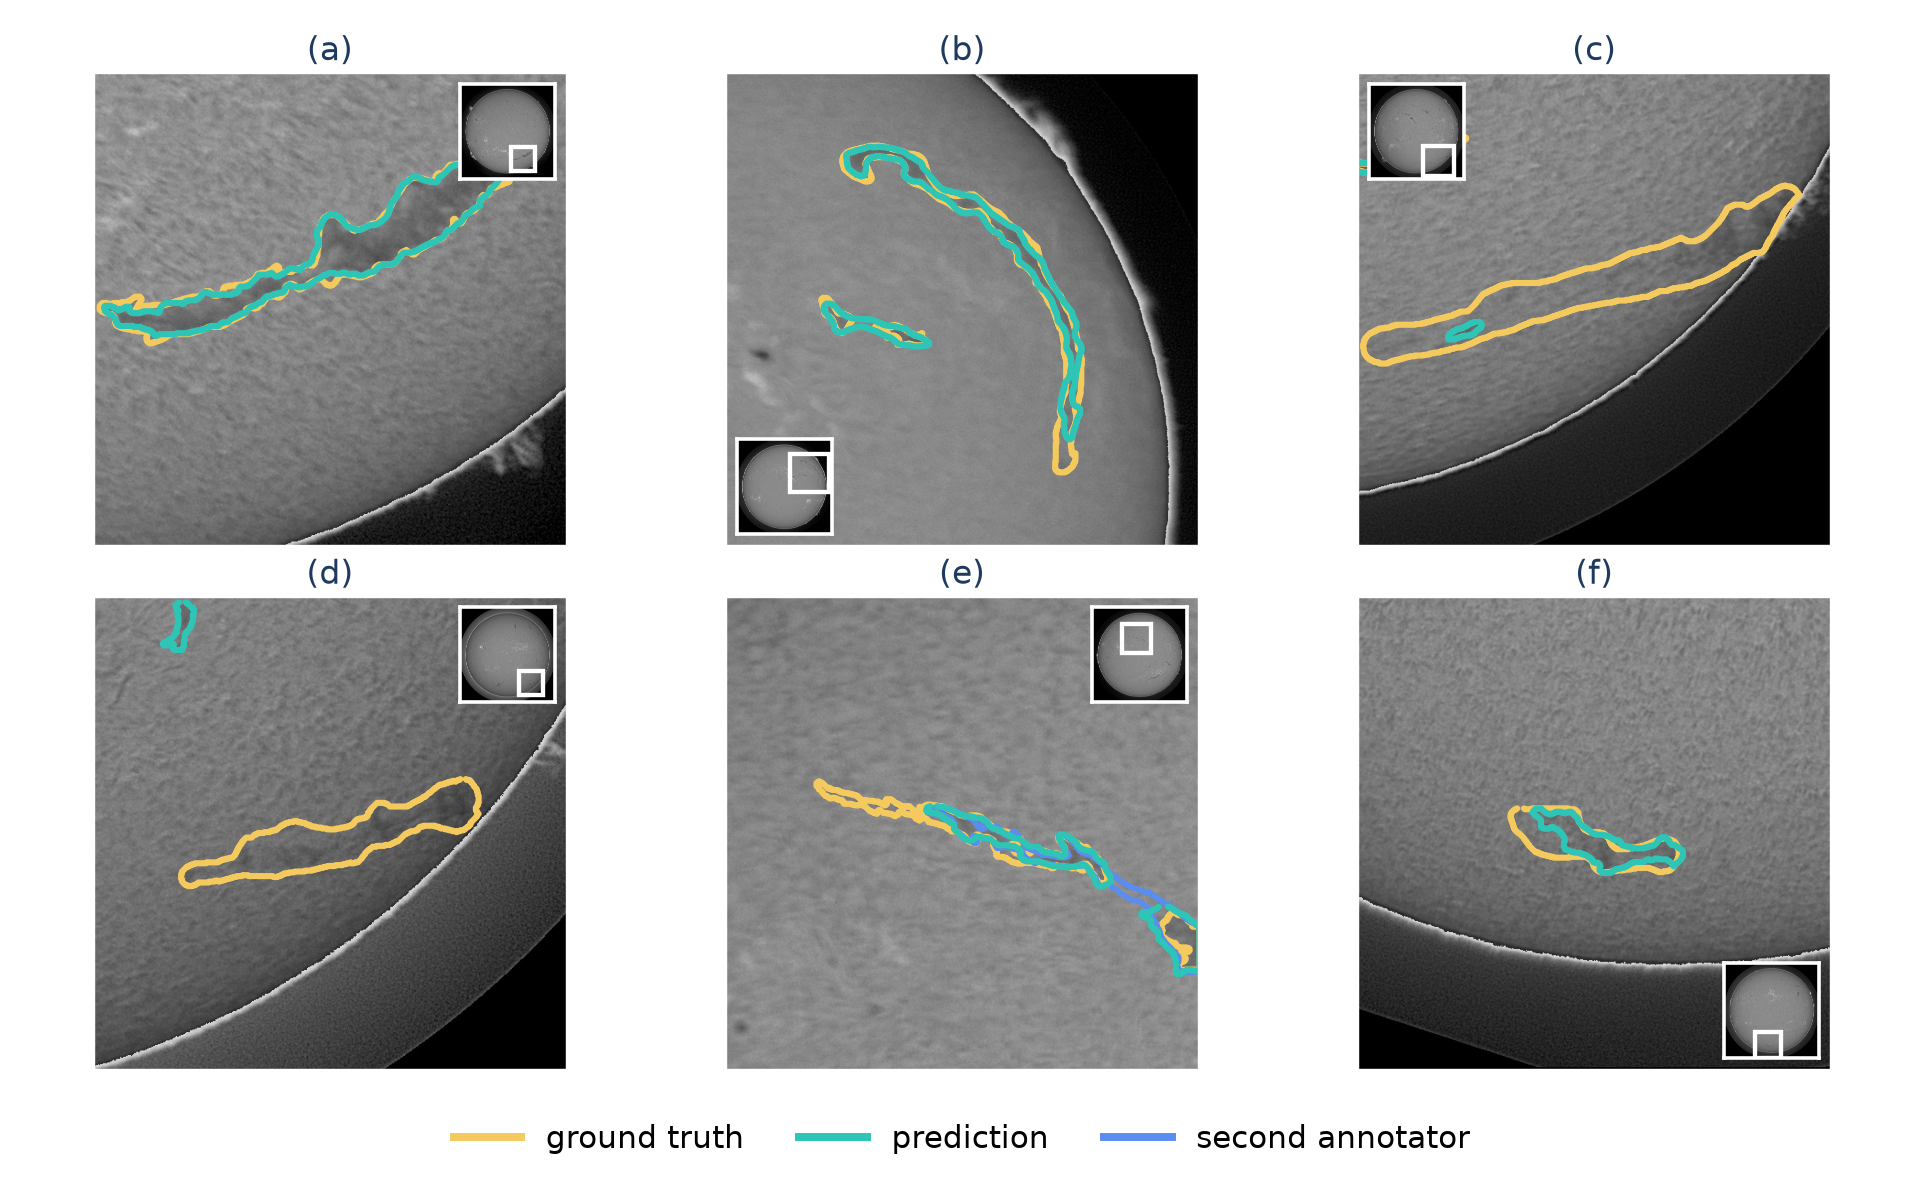
\includegraphics[width=0.68\linewidth]{figures/qualitative.png}
\Description{Six zoomed validation crops in a 3 by 2 grid, each with a full-disk
locator inset and a letter above it. Gold marks the ground truth, teal the
prediction, blue a second annotator. Panels (a,b) follow the annotated filament,
(c,d) miss it, and (e,f) follow one annotator where two disagree.}
\caption{Zoomed validation examples. Gold is the ground truth, teal the
prediction, blue a second annotator. In (a) and (b) the prediction follows thin
barbs and a large curved filament. In (c) and (d) two filaments are missed
outright. In (e) and (f) the annotators disagree and the prediction follows one
of them. Insets locate each crop on the disk.}
\label{fig:qual}
\end{figure*}

\paragraph{Where the speed comes from.}
A full-disk image is four megapixels, and the student is fully convolutional, so
there is no tiling, no patch stitching and no per-image parameter to set. One
pass costs 37\,ms. The KEEP rule and COCO RLE encoding add 34\,ms, which gives
71\,ms end to end, or 14 images per second, for a pipeline that returns
instances rather than a probability map. The earlier version of this pipeline ran
an eight-crop 1024-pixel window, which needs 276\,ms for the forward pass alone,
so a single pass is about seven times cheaper for the same network. All timings
are one RTX~4070 at batch~1 in FP16, averaged over 30 validation images after
warm-up.

\paragraph{Error analysis.}
The remaining error is mostly under-detection. Under the deployed rule the
student has 933 matched instances, 474 false positives and 461 false negatives.
Of the false negatives, 292 (63.3\%) are filaments the model never fires on, 163
(35.4\%) are boundary disagreements with the annotator, and 6 (1.3\%) are two
filaments merged into one prediction. Matched pairs are close, with mean IoU
0.689 and mean Dice 0.813 over the 933 pairs (Fig.~\ref{fig:dist}). Post-hoc
dilation and erosion both lose PQ (dilation by one pixel $-0.025$, by two
$-0.094$, erosion by one $-0.022$), so what remains is not a thin-boundary
problem.

\begin{figure}[t]
\centering
\begin{subfigure}{0.49\linewidth}
  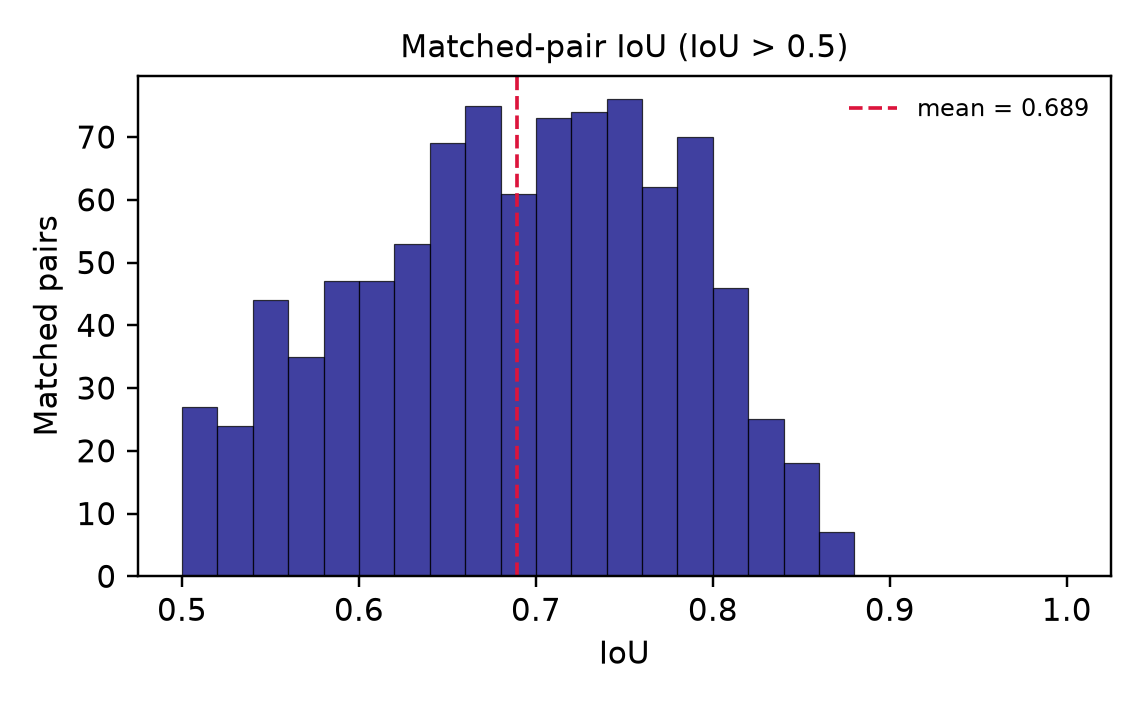
\includegraphics[width=\linewidth]{figures/iou_dist.png}
  \caption{IoU}
\end{subfigure}\hfill
\begin{subfigure}{0.49\linewidth}
  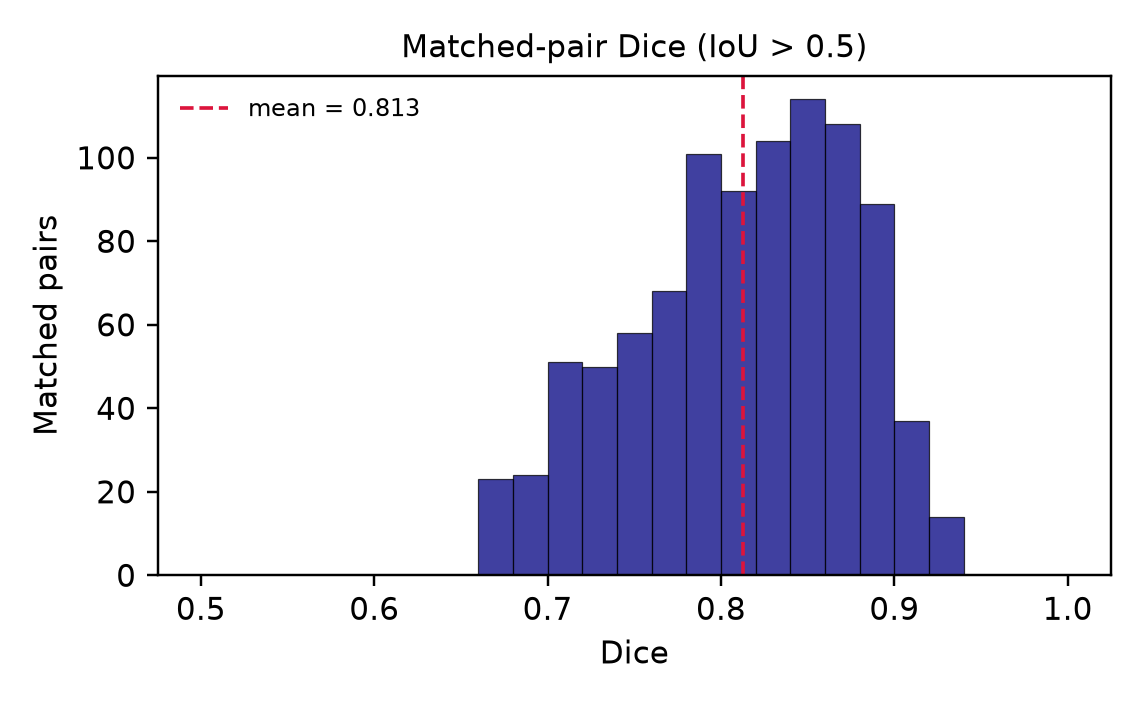
\includegraphics[width=\linewidth]{figures/dice_dist.png}
  \caption{Dice}
\end{subfigure}

\vspace{2pt}
\begin{subfigure}{0.92\linewidth}
  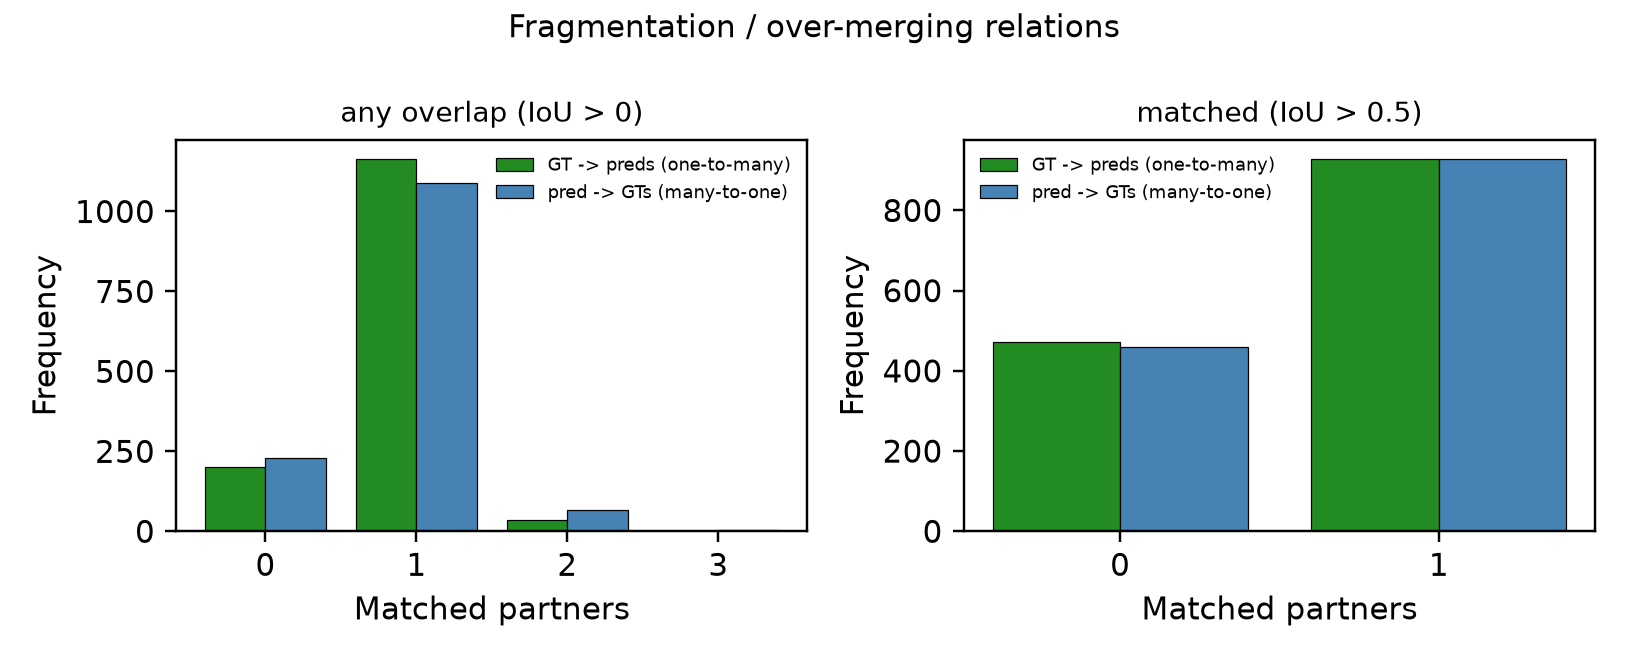
\includegraphics[width=\linewidth]{figures/m2n_dist.png}
  \caption{Overlap partners}
\end{subfigure}
\Description{Three panels: histograms of matched-pair IoU and Dice, and a
two-panel bar chart counting the number of overlap partners per instance at IoU
greater than zero and at IoU greater than 0.5.}
\caption{Matched-pair overlap and partner counts for the submitted student on the
107 validation files. The lower panel counts partners at IoU$>0$ (left) and under
the official IoU$>0.5$ matching (right). Under IoU$>0.5$ every instance has zero
or one partner, so duplicate relations cannot reach the metric.}
\label{fig:dist}
\end{figure}

\paragraph{Fragmentation.}
Under IoU$>0.5$ matching the student has no one-to-many and no many-to-one
relations. That is a property of the matching, which gives each instance at most
one partner, and not a separate result. The informative count is at any overlap.
At IoU$>0$, 2.4\% of ground-truth instances overlap more than one prediction and
5.1\% of predictions overlap more than one ground-truth instance
(Fig.~\ref{fig:dist}, lower panel). The KEEP rule does not act on those
duplicates. It acts on false positives: moving from the older coupled rule to
KEEP changed TP, FP and FN from 916/575/478 to 933/474/461, adding 17 true
positives and removing 101 false positives. Recognition quality rose from 0.635
to 0.666 while segmentation quality moved only from 0.686 to 0.689.

\paragraph{Qualitative comparison.}
Fig.~\ref{fig:qual} shows zoomed validation crops. Panels (a) and (b) contain
the behavior we want, where thin barbs and curved bodies are kept. Panels (c)
and (d) contain the failure we keep seeing, a filament that produces no response
at all. Panels (e) and (f) contain cases where the annotators disagree and the
prediction follows one of them. Limb artifacts do not appear, because the disk
gate removes them before the KEEP rule reads the map.

\paragraph{What the rule and the fine-tunes are worth.}
Table~\ref{tab:ablation} collects the effects we measured with nested 5-fold
cross-validation on the 107 validation files and a paired file-level bootstrap.
The KEEP rule is worth 0.0158 PQ against the older coupled rule, and its interval
is clear of zero. The annotator-sampling fine-tune is worth 0.0127 on a
ConvNeXt-tiny student, and 0.0105 once weight averaging is added. On the
submitted student the same fine-tune is worth 0.0051, and its interval includes
zero, so we do not claim it as a gain. The rule is the one change that moved the
leaderboard on its own.

\begin{table}[t]
\centering
\footnotesize
\setlength{\tabcolsep}{3pt}
\begin{tabular}{@{}lrr@{}}
\toprule
Effect (nested out-of-fold) & $\Delta$PQ & 95\% CI \\
\midrule
KEEP rule vs.\ coupled rule            & $+0.0158$ & [0.0087, 0.0231] \\
ConvNeXt-tiny, annotator sampling      & $+0.0127$ & [0.0045, 0.0217] \\
ConvNeXt-tiny, sampling + averaging    & $+0.0105$ & [0.0032, 0.0177] \\
Submitted student, sampling + averaging & $+0.0051$ & [$-$0.0056, 0.0167] \\
\bottomrule
\end{tabular}
\caption{Paired file-level bootstrap over 4{,}000 resamples for the rule and
fine-tune gains. All intervals are nested 5-fold out-of-fold on the 107
validation files. Each row is a gain over the same model without that change.}
\label{tab:ablation}
\end{table}

\paragraph{A better member does not help the ensemble.}
Adding the fine-tuned student to the four-model ensemble at weights of 0.10,
0.15 and 0.20 moves PQ by $+0.0003$, $-0.0001$ and $+0.0002$, and every interval
spans zero. The same member added at weight 0.10 gives $+0.0001$ ($-0.0024$ to
$+0.0026$). A member can be clearly better on its own and still add nothing,
because all members miss the same unlabeled filaments, so the error that remains
is shared rather than averaged away. That is why we dropped the ensemble from
the submission.

\paragraph{Limitations.}
Three limits bound these numbers. Validation labels are noisy, with an
inter-annotator union-mask IoU of 0.467, and 27\% of our confident detections
match no annotator at all, so absolute validation PQ is optimistic and only
deltas travel. The public leaderboard is rounded to 0.01 and cannot resolve the
effects in Table~\ref{tab:ablation}, which is why we select the accuracy
reference on validation PQ and report intervals rather than absolute levels
alone. The largest untested lever is data coverage, namely five-fold training
over all 707 images instead of 600, rather than a different architecture.

\paragraph{Reproducibility.}
The released package contains the 16.4\,MB student weight, the narrow student
weight, an inference notebook, a 13-check submission verifier and the two timing
scripts behind Fig.~\ref{fig:speed}. The notebook reproduces 0.4591 on the same
107 files. Re-inference over the test set takes about a minute on one GPU and
reproduces 1{,}277 of the 1{,}279 submitted rows byte for byte, with the one
remaining image shifting two contours by a pixel and adding a boundary component
that clears the area test.

% ==================================== %
%              CONCLUSION              %
% ==================================== %
\section{Conclusion}
    We submitted a 4.28\,M-parameter network that processes a full-disk
    H-$\alpha$ image in 37\,ms and scores 0.38 on the public leaderboard, the
    same as a 171\,M four-model ensemble that is 9.5 times slower. Most of the
    accuracy we found was in post-processing. Letting the contour threshold and
    the instance-acceptance test be set independently was worth 0.0158 PQ and one
    leaderboard step on its own, with no retraining. Training on every annotator
    and averaging the last epochs gave a smaller and less certain gain. What
    remains is under-detection on faint, low-contrast filaments, which points to
    more training data rather than a different architecture.


% ==================================== %
%            ACKNOWLEDGMENT            %
% ==================================== %
\section{Acknowledgment}\label{sec:acknowledgment}
\begingroup\sloppy
    The Filament Segmentation Challenge 2026 is sponsored by the U.S. National
    Science Foundation (NSF) National Solar Observatory (NSO) and its organization
    is partially supported by NSF grants 2209912, 2433781 and 2511630 (CISE/CSE,
    OAC, and AST/MPS).

    This work utilizes GONG data obtained by the NSO Integrated Synoptic Program,
    managed by the National Solar Observatory, which is operated by the Association
    of Universities for Research in Astronomy (AURA), Inc. under a cooperative
    agreement with the National Science Foundation and with contribution from the
    National Oceanic and Atmospheric Administration. The GONG network of instruments
    is hosted by the Big Bear Solar Observatory, High Altitude Observatory,
    Learmonth Solar Observatory, Udaipur Solar Observatory, Instituto de Astrofísica
    de Canarias, and Cerro Tololo Interamerican Observatory.
\endgroup

\bibliographystyle{ACM-Reference-Format}
\bibliography{main}

\end{document}
